%!TEX root = ../template.tex
\typeout{NT FILE appendix-prototypes.tex}%
% REQUIRES \usepackage{float} in the preamble (or template.tex) for the
% [H] figure placement used throughout this file. [H] (capital, from the
% float package) forces each figure to render exactly where it is written
% in the source, with no floating to a later page — unlike the default
% [h] (lowercase), which is only a placement *hint* that LaTeX is free to
% override whenever a figure doesn't fit, which is what was causing
% captions and figures to separate onto different pages.

\chapter{Case-Study Wall Comparison}
\label{app:case-comparison}

Table~\ref{tab:case-comparison} expands the three-wall comparison
summarised in \S\ref{sec:pw-domain} with the full set of properties
compared across the Grande Panorama de Lisboa, Chafariz Velho, and the
Alto de Santa Catarina mural.

\begin{table}[h]
\centering
\caption{Comparison of the three case-study surfaces used throughout this thesis.}
\label{tab:case-comparison}
\small
\resizebox{\textwidth}{!}{%
\begin{tabular}{p{3.6cm}p{4.4cm}p{4.4cm}p{4.4cm}}
\toprule
 & \textbf{Grande Panorama de Lisboa} & \textbf{Chafariz Velho} & \textbf{Alto de Santa Catarina Mural} \\
\midrule
Role in thesis & Central motivating case & Primary development/test case & Generalisability test case \\
Length & $\sim$23\,m & $\sim$30--40\,m (estimated) & $\sim$30--40\,m \\
Geometry & U-shaped (needs $x,y,z$) & Circular (needs $x,y,z$ + yaw) --- and the wall is not vertical so needs also Pitch and Roll & Two planar faces at $\sim$120° (needs $x,y$ + yaw across the join) \\
Setting & Indoor, controlled lighting & Outdoor, variable light/shadow & Outdoor, variable light/shadow \\
Content type & Built city (buildings) & Historical scenes/figures & Wildlife/biodiversity \\
Status axis & Earthquake fate (4 states) & Wall-specific, non-earthquake & \textbf{None --- absent by design} \\
Public access during thesis & Closed since Nov.\ 2025 (PRR works) & Permanently accessible & Permanently accessible \\
\bottomrule
\end{tabular}
}
\end{table}

\chapter{UI Design Prototypes}
\label{app:prototypes}

This appendix collects the visual design exploration and screen-level
prototypes referenced from \S\ref{subsec:pw-core-concept} and
\S\ref{sec:wp-completed}. All of it predates the Unity decision
(\S\ref{sec:pw-techstack}) and was built in Flutter as design exploration,
not as code intended to carry forward; what carries forward is
the visual language and interaction logic shown here, not the
implementation.

\section{Core User Flow}
\label{app:user-flow}

Figure~\ref{fig:user-flow} traces the main interaction paths once inside
the AR view. A visitor completes onboarding, the camera scans and locks
onto the wall, and points of interest appear with three next steps on
offer: tapping a marker for its content card, opening the timeline, or
picking a guided circuit.

\begin{figure}[H]
\centering
\resizebox{\textwidth}{!}{%
\begin{tikzpicture}[
  node distance=1.1cm and 2.6cm,
  every node/.style={font=\small},
  box/.style={draw, rounded corners, align=center, minimum width=3.1cm, minimum height=0.9cm, fill=gray!6}
]
  \node[box] (onboard) {Onboarding \\ (profile + permission)};
  \node[box, below=of onboard] (scan) {Camera opens \\ Wall scan/lock};
  \node[box, below=of scan] (markers) {POI markers appear};
  \node[box, below left=of markers, xshift=-1.2cm] (card) {Tap POI $\to$ \\ content card};
  \node[box, below=of markers] (timeline) {Activate timeline \\ $\to$ drag slider};
  \node[box, below right=of markers, xshift=1.2cm] (circuit) {Select circuit $\to$ \\ guided sequence};
  \node[box, below=of circuit] (quiz) {Knowledge check \\ $\to$ badge};

  \draw[->, thick] (onboard) -- (scan);
  \draw[->, thick] (scan) -- (markers);
  \draw[->, thick] (markers) -- (card);
  \draw[->, thick] (markers) -- (timeline);
  \draw[->, thick] (markers) -- (circuit);
  \draw[->, thick] (circuit) -- (quiz);
\end{tikzpicture}%
}
\caption{Main user flows from onboarding through the three core interaction branches: free exploration, the timeline, and a guided circuit.}
\label{fig:user-flow}
\end{figure}

















\section{Visual Style Exploration}
\label{app:style-exploration}
 
Two distinct visual directions were prototyped end-to-end, each in a
light and a dark variant, before either was locked into the design
tokens described in \S\ref{sec:wp-completed}. The first, called here
\textbf{Editorial Luxury}, pairs a warm ivory/parchment surface with deep
navy content cards and gold-to-amber accents, using an italic serif
display face for landmark names (``The \emph{Royal} Galleon'') and
museum-label-style metadata rows (location, period, tile count,
rarity). It reads more like a high-end exhibition catalogue than a
mobile game, which was the point. The second, \textbf{Aurora}, leans
into a bluer, more tech-flavoured palette instead.
Figures~\ref{fig:style-luxury-light}/~\ref{fig:style-luxury-dark} and
Figure~\ref{fig:style-aurora-light}/~\ref{fig:style-aurora-dark} show
each direction in both variants.
 
\begin{figure}[H]
\centering
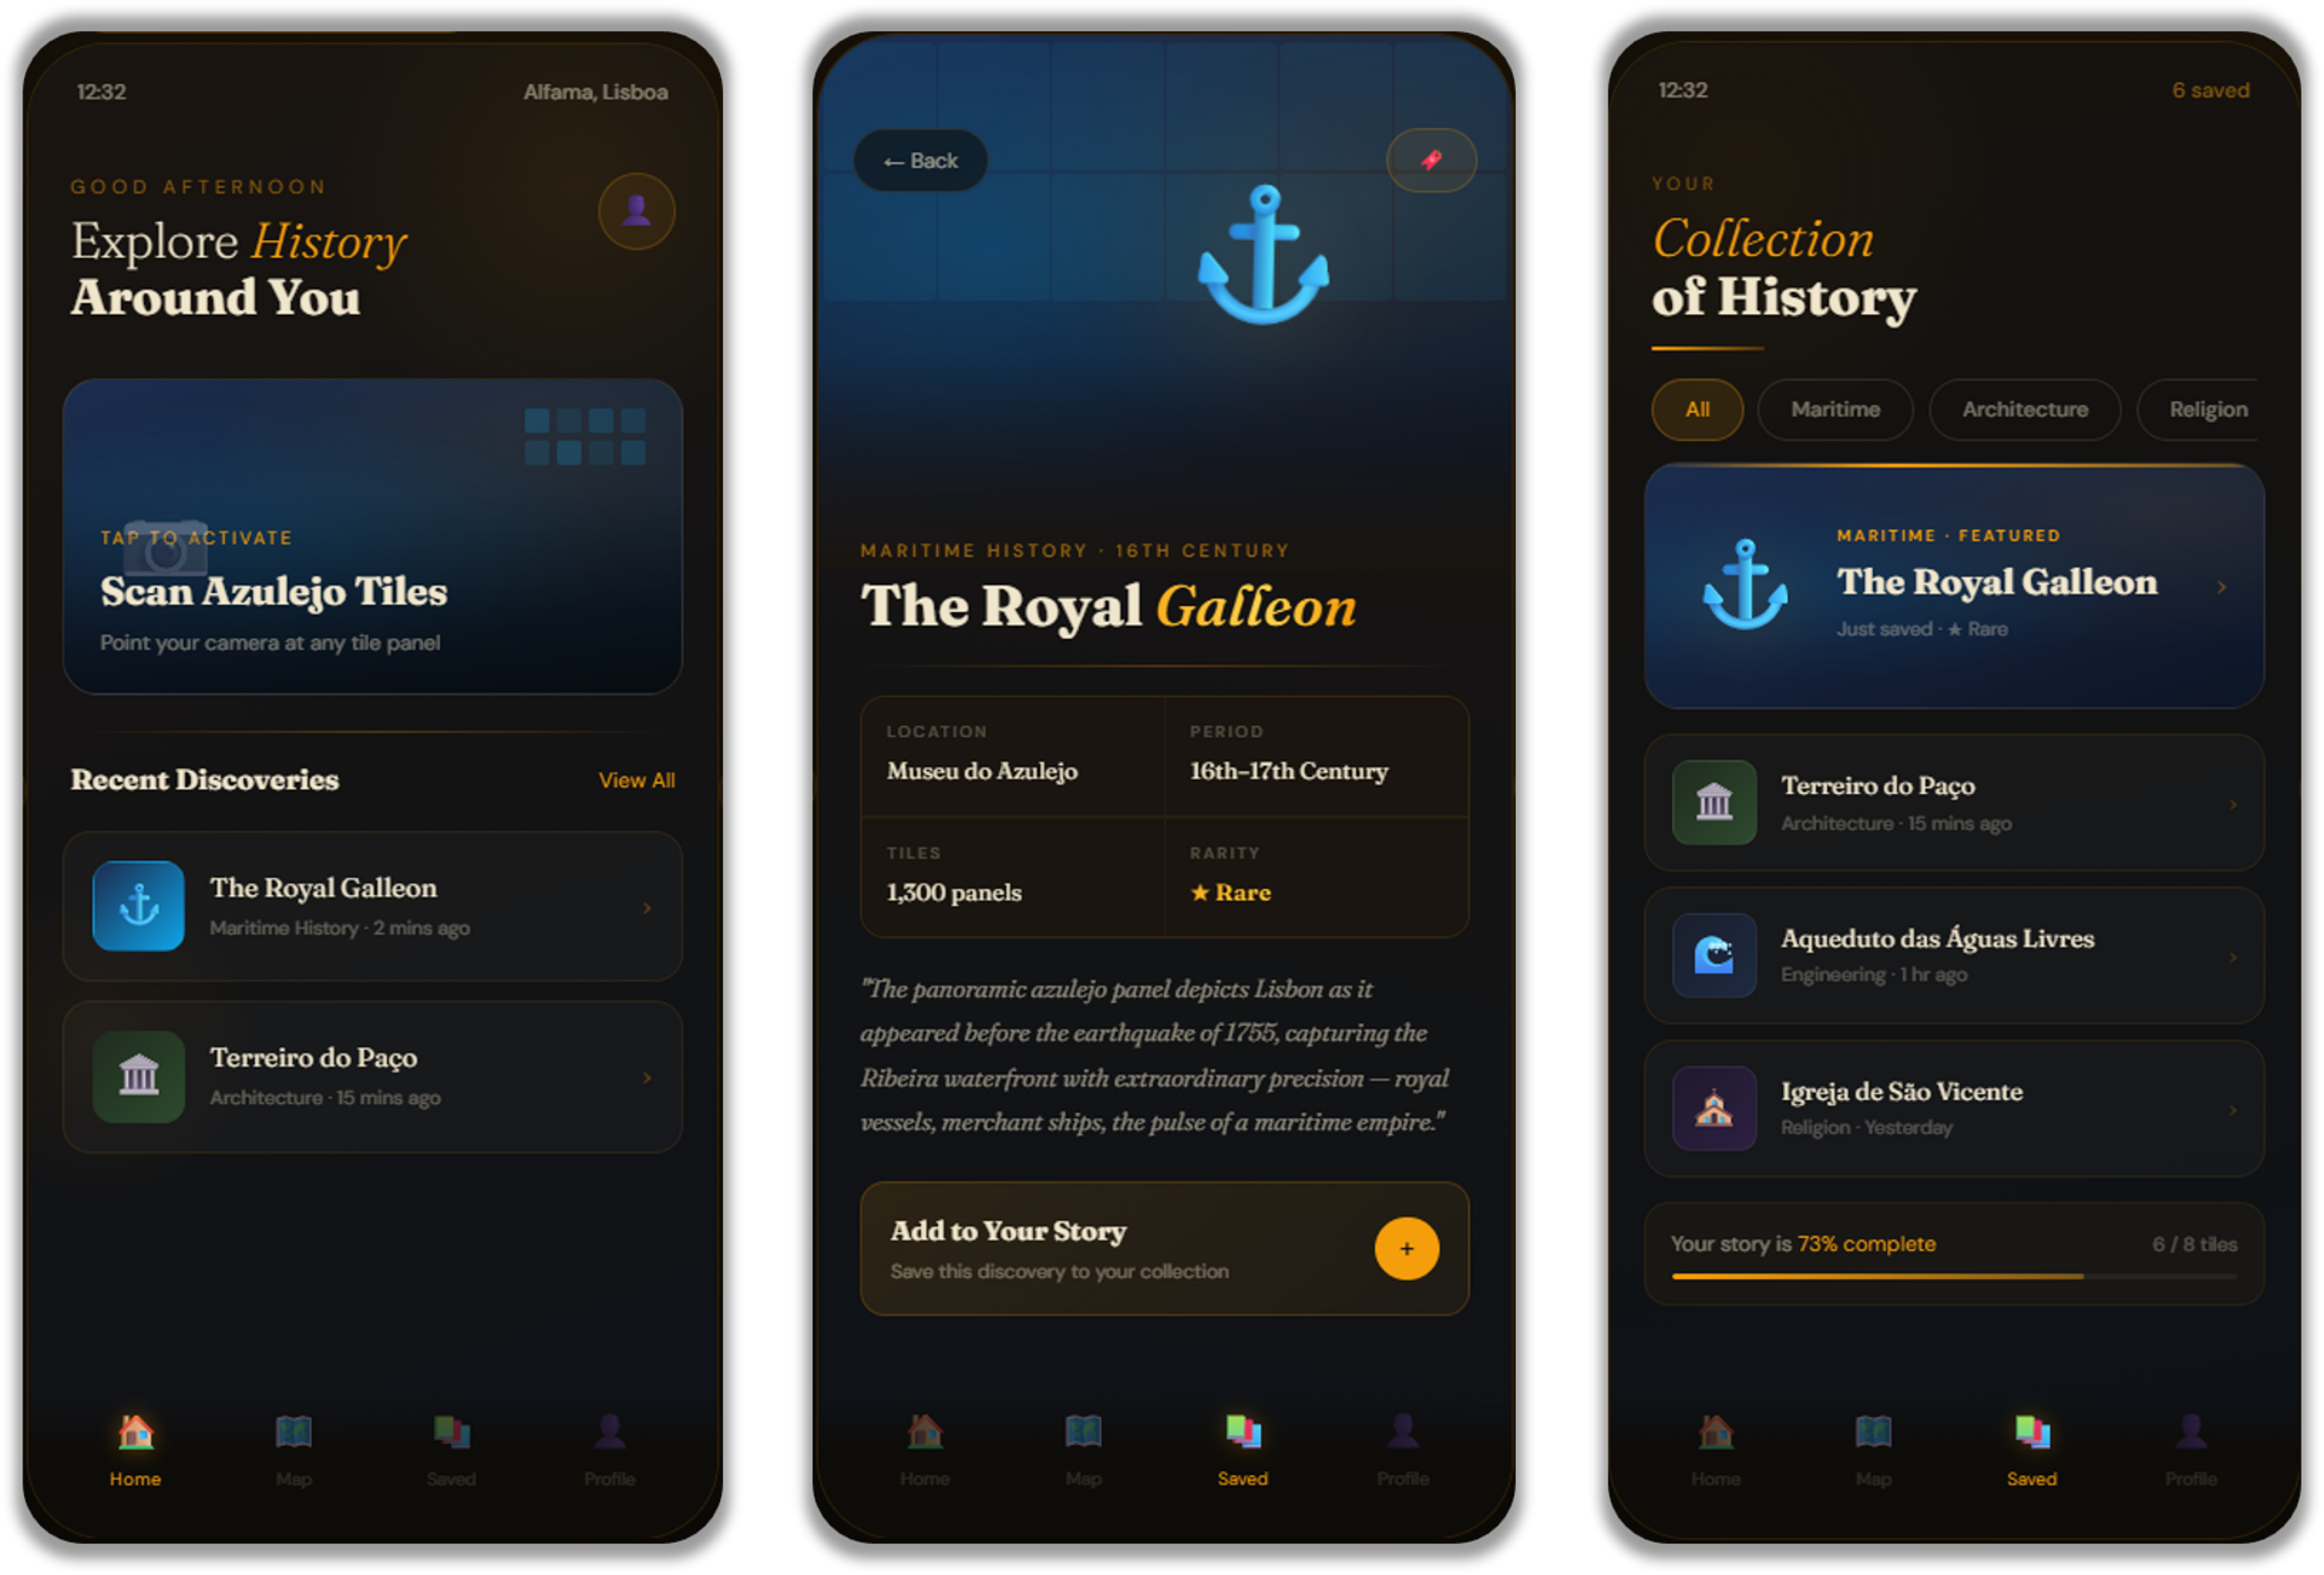
\includegraphics[width=0.95\textwidth]{5-Figures/my_figures/style_stone_and_gold_dark.png}
\caption{``Stone \& Gold Luxury'' style direction, dark variant.}
\label{fig:style-luxury-dark}
\end{figure}

\begin{figure}[H]
\centering
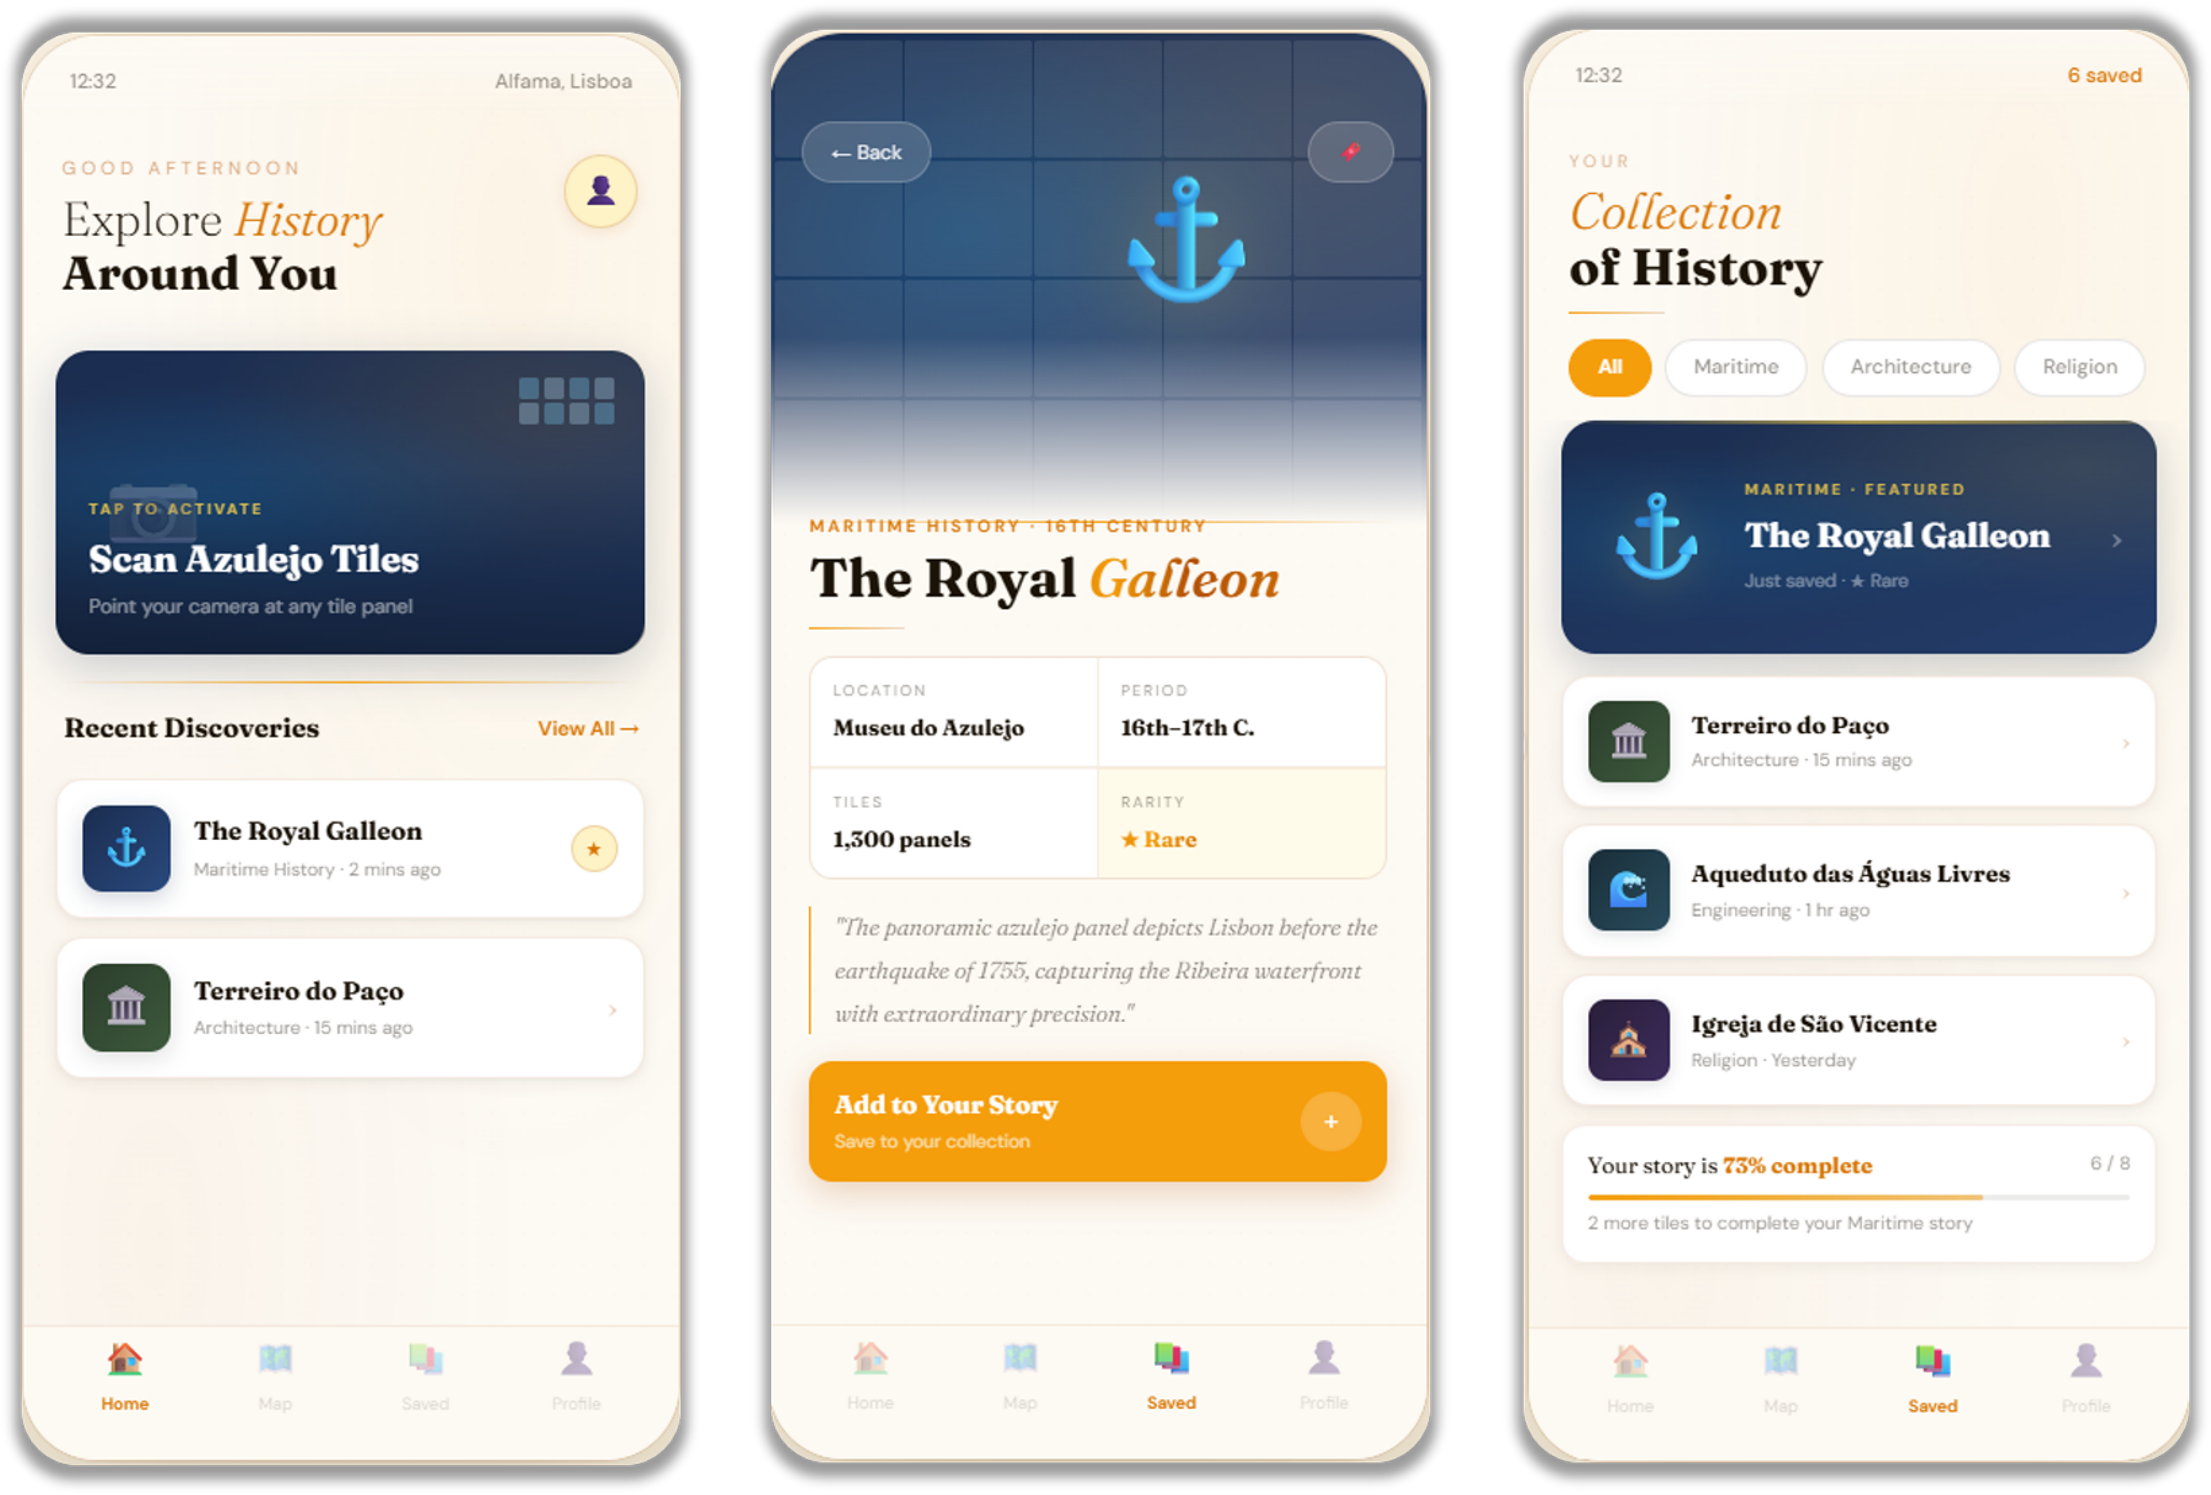
\includegraphics[width=0.95\textwidth]{5-Figures/my_figures/style_stone_and_gold_light.png}
\caption{``Stone \& Gold Luxury'' style direction, light variant.}
\label{fig:style-luxury-light}
\end{figure}

 
\begin{figure}[H]
\centering
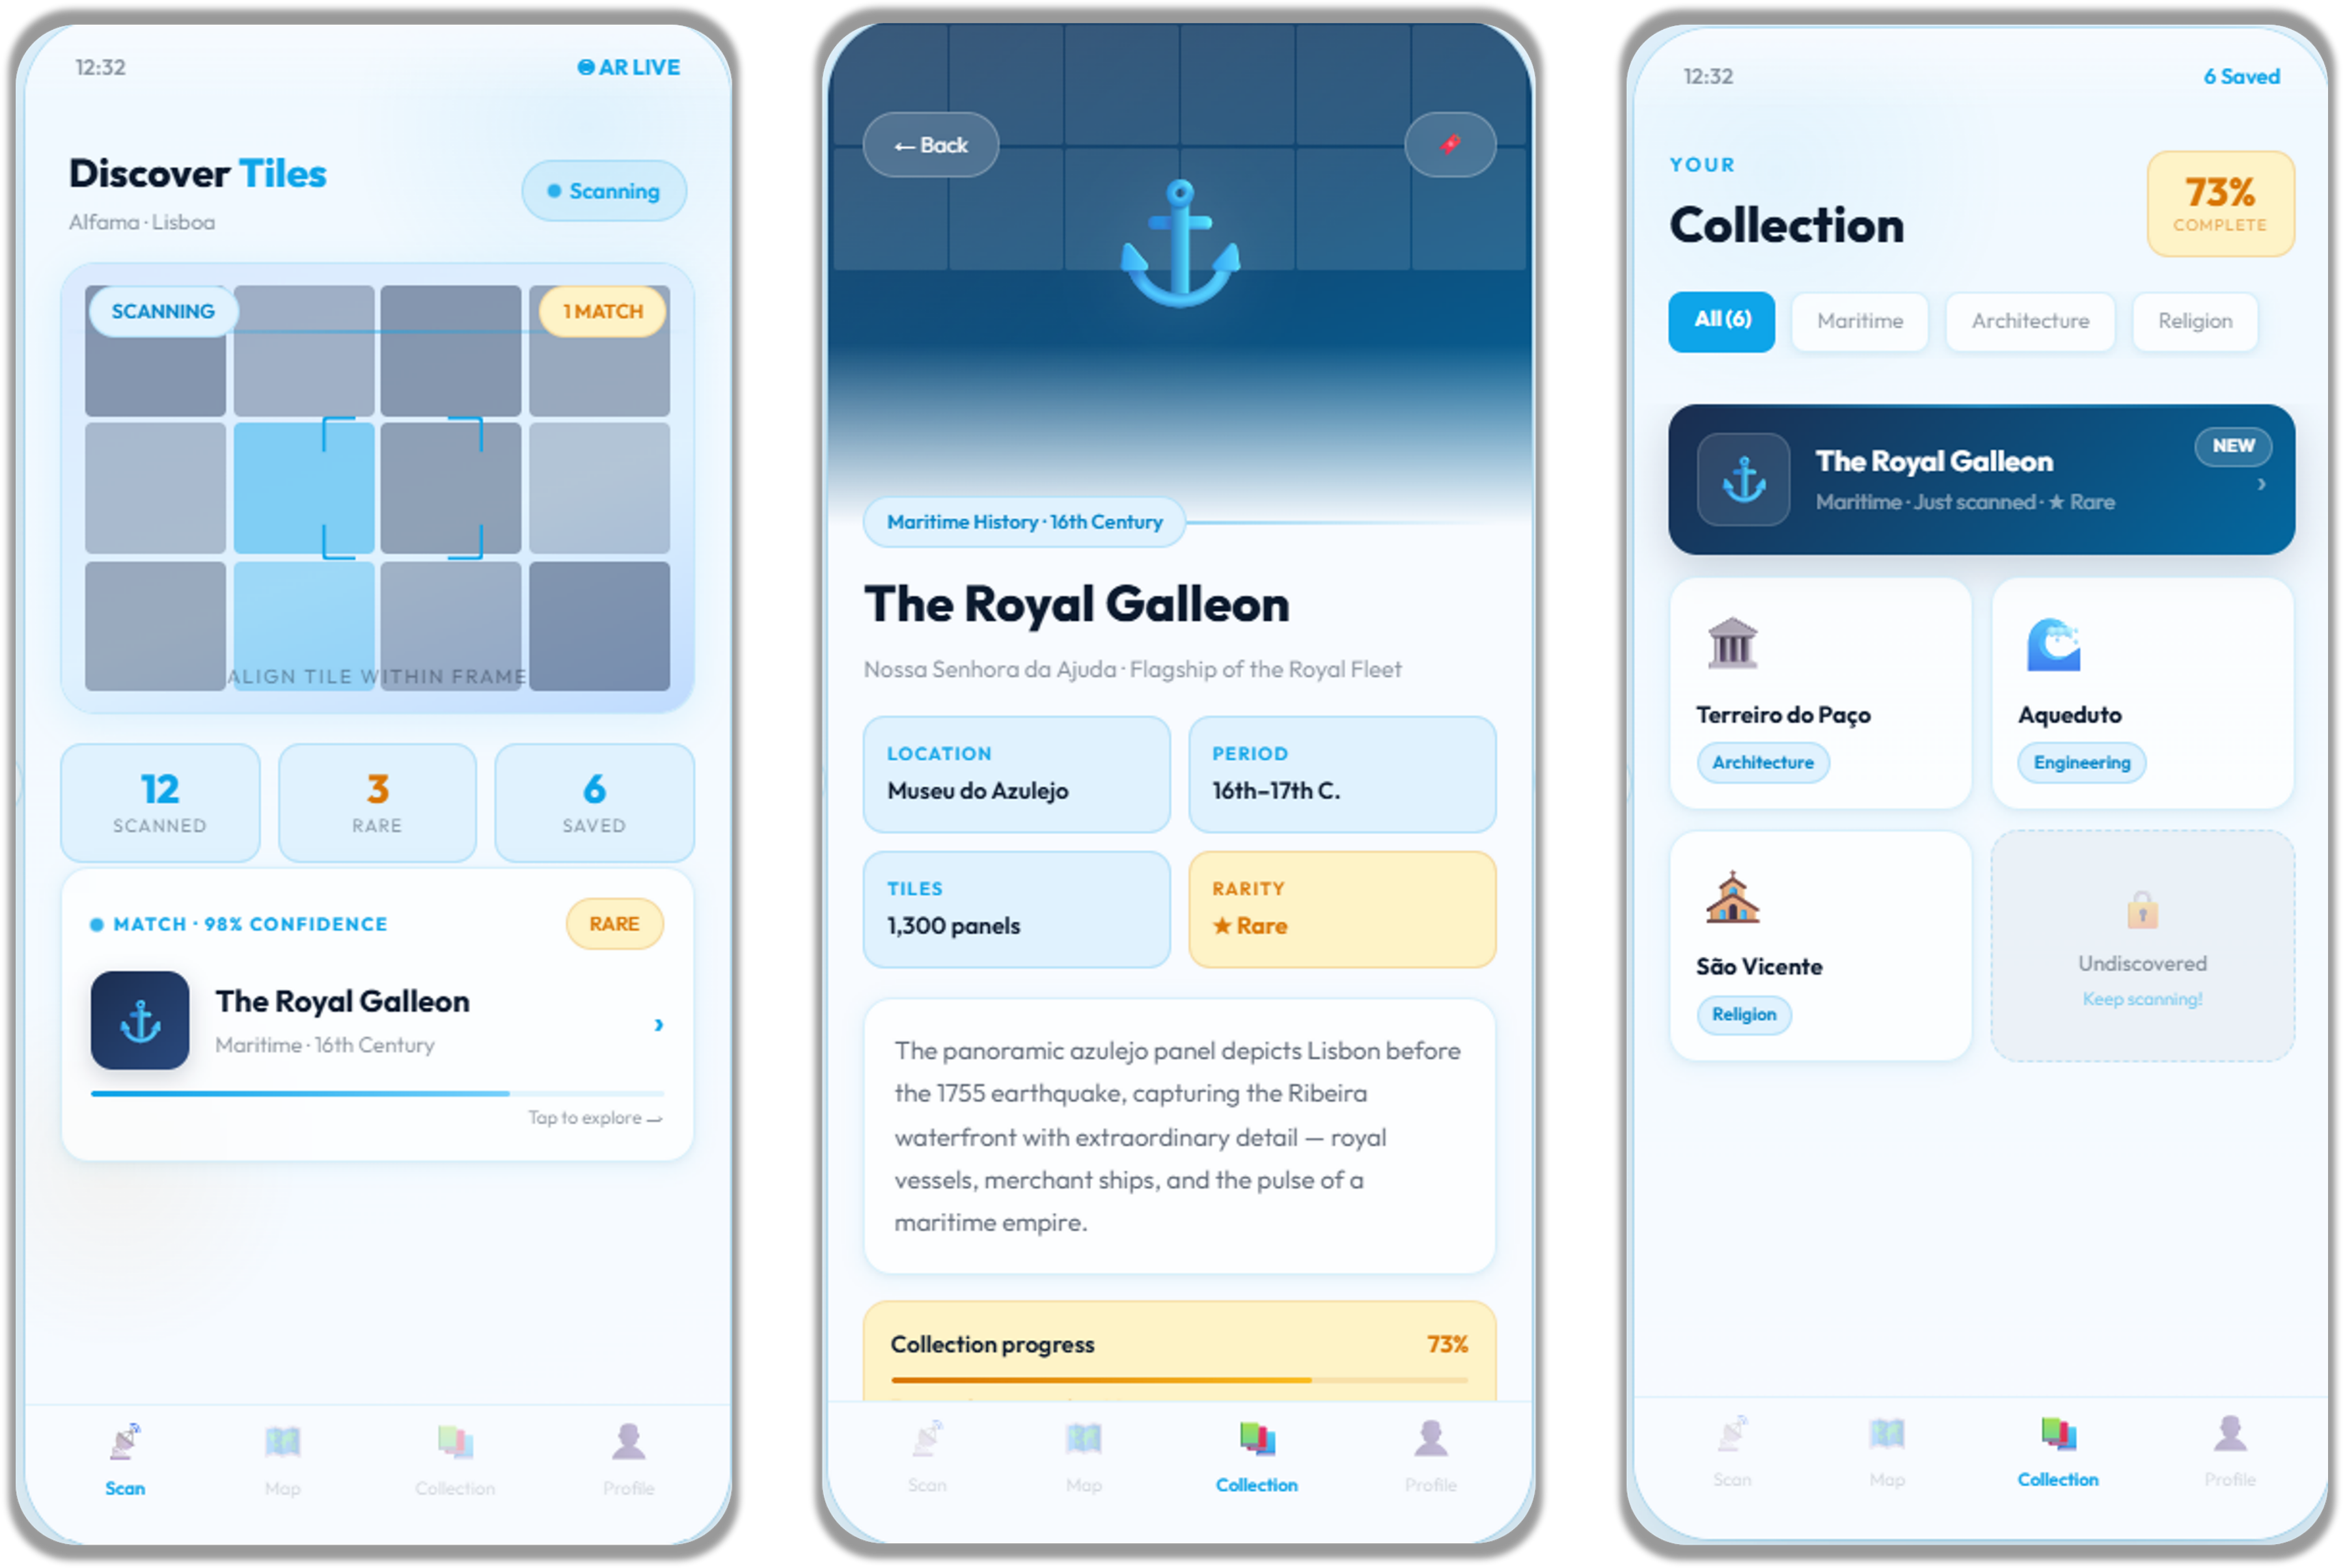
\includegraphics[width=0.95\textwidth]{5-Figures/my_figures/style_aurora_light.png}
\caption{``Aurora'' style direction, light variant.}
\label{fig:style-aurora-light}
\end{figure}

\begin{figure}[H]
\centering
\includegraphics[width=0.95\textwidth]{5-Figures/my_figures/style_aurora_dark.png}
\caption{``Aurora'' style direction, dark variant.}
\label{fig:style-aurora-dark}
\end{figure}

 
 
Editorial Luxury is the direction that was carried forward into the
production design system (\S\ref{sec:wp-completed}). The choice follows
from the principle in \S\ref{subsec:pw-core-concept} that the interface
should mediate the heritage artefact, not compete with it for
attention. Aurora's tech-blue style suits a gamified collection
mechanic well, but it ends up framing the experience as a scanning game
first and a heritage encounter second, which is the wrong emphasis
here. Editorial Luxury's restraint (muted tones, archival-style
metadata, no game-like chrome over the camera view) keeps that framing
the other way around, and that matters more for an app whose stated
purpose is historical interpretation, not collecting things for their
own sake. Aurora's scan-and-match interaction pattern and its
rarity/collection mechanic were not thrown out, though; both inform the
gamification features described in \S\ref{subsec:pw-feature-phases},
just dressed in Editorial Luxury's calmer visual language instead of
Aurora's own.
















\section{POI Marker Encoding System}
\label{app:poi-markers}

The marker system encodes two variables independently, so that neither
competes with the other for the same visual channel: a point of
interest's category is carried by fill colour and icon, while its
earthquake fate is carried independently by border colour and style,
ranging from a solid green border for structures that survived intact
through progressively shorter dashes to a dotted border for total loss.
Figure~\ref{fig:poi-legend} shows this encoding in the abstract, as
presented to a visitor through the in-app legend.

\begin{figure}[H]
\centering
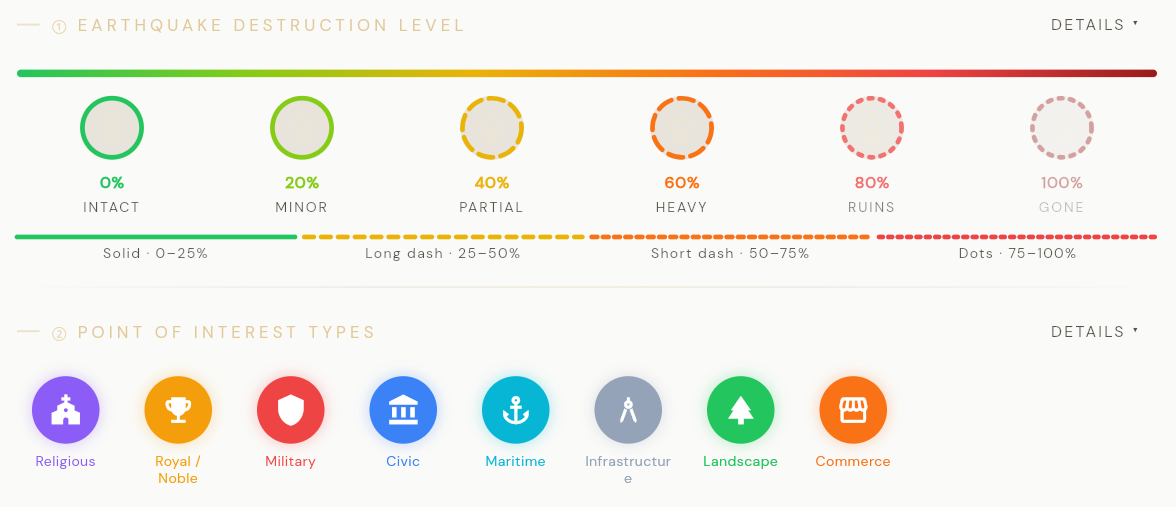
\includegraphics[width=0.95\textwidth]{5-Figures/my_figures/POI_Markers_Labels.png}
\caption{POI marker legend: the earthquake destruction spectrum (border colour and style, six levels from intact to vanished) and the point-of-interest type taxonomy (fill colour and icon, eight categories) as two independent encoding channels.}
\label{fig:poi-legend}
\end{figure}

This follows directly from the
Core/Walls separation in \S\ref{sec:pw-architecture}: the eight
categories and their colour/icon mapping in Figure~\ref{fig:poi-legend}
are \emph{wall-specific content}, not part of the Core encoding logic.
They were designed around the Grande Panorama, which depicts a built
city, so religious, royal, military, and civic structures are categories
that actually make sense for a skyline. Chafariz Velho's azulejo scenes
depict historical episodes and personalities, not
buildings, so a future wall built around it (or around any similarly
non-architectural heritage surface) would need its own taxonomy
entirely: a different set of categories, colours, and icons, defined in
that wall's own data, reusing the same dual-channel marker mechanism
(category on one channel, a status or fate dimension on the other)
without touching Core code. The encoding \emph{pattern} generalises. 

Figure~\ref{fig:poi-map} shows the same system applied in context on the
Grande Panorama, and it surfaces a second design detail that isn't
visible in the legend alone: markers carry a visual hierarchy of
importance, not just a flat encoding. Higher-priority points of interest,
named landmarks such as Castelo de S\~{a}o Jorge, S\'{e} de Lisboa, or
Pal\'{a}cio Pombal, render as larger markers with a visible category icon
and a text label, while lower-priority points render as small,
unlabelled, colour-only dots that still carry the category and fate
encoding but don't compete for attention at the same visual weight. This
is a fairly direct implementation of the level-of-detail principle
motivated by RQ2 (\S\ref{sec:pw-problem-rq}) and the legibility findings
discussed in \S\ref{subsec:rw-visitor-models}: with well over a hundred
points of interest on a single wall, a flat, equally-weighted marker
field simply would not be readable, so importance has to be rendered,
not just implied. The open content card for Igreja de Santa Engr\'{a}cia
restates the same two-channel encoding as text (``Religioso,''
``Intacto'') alongside a short narrative note (construction begun in
1682 and only completed in 1966, the building survived the 1755
earthquake intact), so the colour-and-icon signal is never the only
carrier of meaning for visitors who cannot, or choose not to, rely on
colour alone.

\begin{figure}[H]
\centering
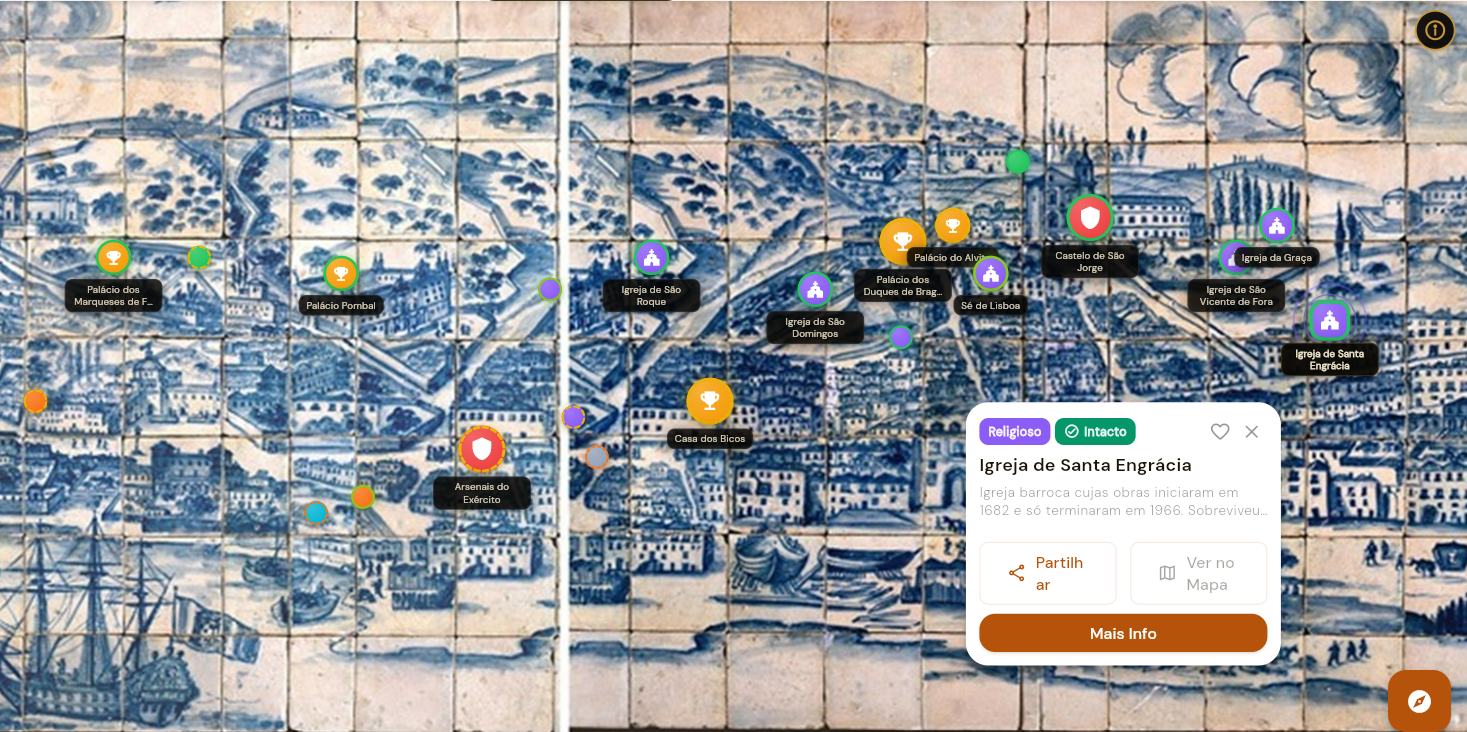
\includegraphics[width=0.95\textwidth]{5-Figures/my_figures/POI_Markers_Display.png}
\caption{POI markers in context on the Grande Panorama, showing the importance hierarchy (large labelled icons for priority POIs, small unlabelled dots for secondary POIs) and the content card's text restatement of the marker encoding for Igreja de Santa Engr\'{a}cia.}
\label{fig:poi-map}
\end{figure}





































\chapter{Development Timeline}
\label{app:gantt}

Figure~\ref{fig:gantt} lays the six phases introduced in
\S\ref{subsec:pw-feature-phases} and scheduled in \S\ref{sec:wp-overview}
against a six-month calendar. It uses relative month labels (M1--M6)
instead of fixed dates, since the confirmed start date still depends on
supervisor sign-off following this report. The stretch phase is drawn
with a dashed outline: time-permitting, not committed.

\begin{figure}[H]
\centering
\resizebox{\textwidth}{!}{%
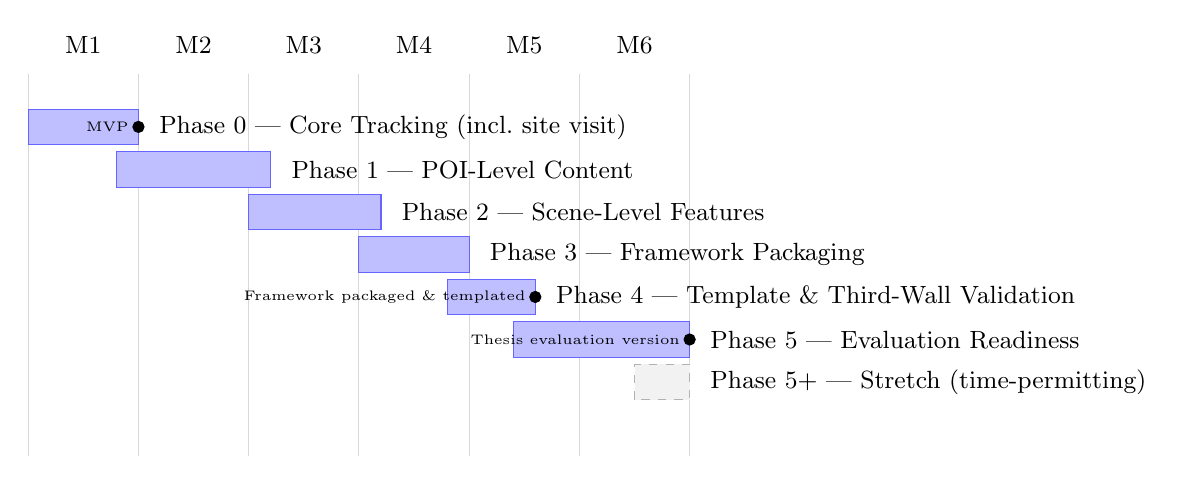
\begin{tikzpicture}[x=1.4cm, y=0.9cm]
  % Month gridlines
  \foreach \m in {0,...,6} {
    \draw[gray!30] (\m,0) -- (\m,-5.4);
  }
  \foreach \m [count=\i from 0] in {M1,M2,M3,M4,M5,M6} {
    \node[font=\small] at (\i+0.5,0.4) {\m};
  }
 
  % Phase bars: (start, end, row, label, color)
  \draw[fill=blue!25, draw=blue!60] (0,-1) rectangle (1.0,-0.5);
  \node[anchor=west, font=\small] at (1.1,-0.75) {Phase 0 --- Core Tracking (incl.\ site visit)};
 
  \draw[fill=blue!25, draw=blue!60] (0.8,-1.6) rectangle (2.2,-1.1);
  \node[anchor=west, font=\small] at (2.3,-1.35) {Phase 1 --- POI-Level Content};
 
  \draw[fill=blue!25, draw=blue!60] (2.0,-2.2) rectangle (3.2,-1.7);
  \node[anchor=west, font=\small] at (3.3,-1.95) {Phase 2 --- Scene-Level Features};
 
  \draw[fill=blue!25, draw=blue!60] (3.0,-2.8) rectangle (4.0,-2.3);
  \node[anchor=west, font=\small] at (4.1,-2.55) {Phase 3 --- Framework Packaging};
 
  \draw[fill=blue!25, draw=blue!60] (3.8,-3.4) rectangle (4.6,-2.9);
  \node[anchor=west, font=\small] at (4.7,-3.15) {Phase 4 --- Template \& Third-Wall Validation};
 
  \draw[fill=blue!25, draw=blue!60] (4.4,-4.0) rectangle (6.0,-3.5);
  \node[anchor=west, font=\small] at (6.1,-3.75) {Phase 5 --- Evaluation Readiness};
 
  \draw[dashed, fill=gray!10, draw=gray!60] (5.5,-4.6) rectangle (6.0,-4.1);
  \node[anchor=west, font=\small] at (6.1,-4.35) {Phase 5+ --- Stretch (time-permitting)};
 
  % Milestone markers
  \draw[fill=black] (1.0,-0.75) circle (2pt);
  \node[anchor=east, font=\tiny] at (1.0,-0.75) {MVP};
  \draw[fill=black] (4.6,-3.15) circle (2pt);
  \node[anchor=east, font=\tiny] at (4.6,-3.15) {Framework packaged \& templated};
  \draw[fill=black] (6.0,-3.75) circle (2pt);
  \node[anchor=east, font=\tiny] at (6.0,-3.75) {Thesis evaluation version};
\end{tikzpicture}%
}
\caption{Six-month development timeline. Phase boundaries overlap by design, so evaluation findings from one phase can feed into the next before it fully begins.}
\label{fig:gantt}
\end{figure}




















\chapter{Full Risk Analysis}
\label{app:risks}

Table~\ref{tab:risks} expands the risk summary given in
\S\ref{sec:wp-risks} with the secondary risks (licensing, tooling
effort, recruitment, content pacing, and risks specific to the
framework's generalisability claim) that matter for week-to-week
planning but are less central to the thesis's core claims than the
access- and ethics-related risks discussed in the main text.

\begin{table}[h]
\centering
\caption{Principal risks to the development plan and their mitigations.}
\label{tab:risks}
\small
\resizebox{\textwidth}{!}{%
\begin{tabular}{p{4.2cm}p{1.5cm}p{1.4cm}p{6.3cm}}
\toprule
\textbf{Risk} & \textbf{Likelihood} & \textbf{Impact} & \textbf{Mitigation} \\
\midrule
Cannot access Grande Panorama for reference photography while MNAz is closed & High & Medium & Continue treating Chafariz Velho and the mural wall as fully sufficient case studies (\S\ref{subsec:pw-chafariz}, \S\ref{subsec:pw-generalisability}); capture Panorama photography opportunistically if any supervised access becomes possible \\
MNAz does not reopen before submission & High & Low & Already designed around: no contribution claim or evaluation in \S\ref{sec:pw-problem-rq}/\S\ref{sec:pw-evaluation} depends on MNAz access \\
Unity UI tooling proves slower than estimated for content-heavy screens & Medium & Medium & Reassess after Phase~1; fall back to a leaner UI scope instead of reintroducing Flutter mid-project \\
Recruitment for evaluation falls short of planned N (\S\ref{sec:pw-evaluation}) & Medium & Medium & Treat the 20--30 target as a ceiling, not a threshold, and report whatever N is actually achieved \\
Content production (POI text across 4 profiles) falls behind schedule & Medium & High & No new POI is added to a wall's dataset until existing POIs' content across all profiles is complete \\
Ethics approval for street-recruited evaluation is not yet requested & Medium & High & Submit the request in Phase~0, alongside tracking work, before content production is finished \\
Framework engineering drifts into speculative generality beyond what any case study actually needs & Medium & Medium & Every architectural feature must trace to a concrete requirement from one of the three walls (\S\ref{subsec:pw-generalisability}); features that do not are deferred past submission \\
\bottomrule
\end{tabular}
}
\end{table}